\begin{surferPage}[216 Singularities]{سطوح ذات متفردات حقيقية عديدة}
كما سبق وذكرنا، العدد الأقصى $\mu(7)$ لمتفردات سطح درجته $7$ غير معروف بالتحديد. كل ما لدينا هو حد أعلى وحد أدنى: $99\le \mu(7) \le 104$.

   ليس مفاجئاً إذاً أن نعرف الأقل بكثير عن درجة  $d$ عامة.
    على الأقل، تمكن كل من سونيا بريسك
    \textenglish{(Sonja Breske)}
     وأوليفر لابس
      \textenglish{\mbox{(Oliver~Labs)}}
       ودوكو فان ستراتن
        \textenglish{(Duco van~Straten)}
         من ملاءمة بناء من إس في شموتوف
         \textenglish{(S.V.\ Chmutov)}
         بحيث أن عدد المتفردات الأقصى الحالي تحققه أيضاً السطوح ذات المتفردات الحقيقية.
    إلى اليوم نعرف:
    \[0,41\bar{6}d^3 \lessapprox \mu(d) \lessapprox 0.44\bar{4} d^3.\]
    من أعلاه، يمكننا أن نرى تناظر البناء والعلاقة مع العدد الأقصى للبقع السوداء في ترتيب الخطوط:
    \begin{center}
      \begin{tabular}{c@{\qquad}c}
        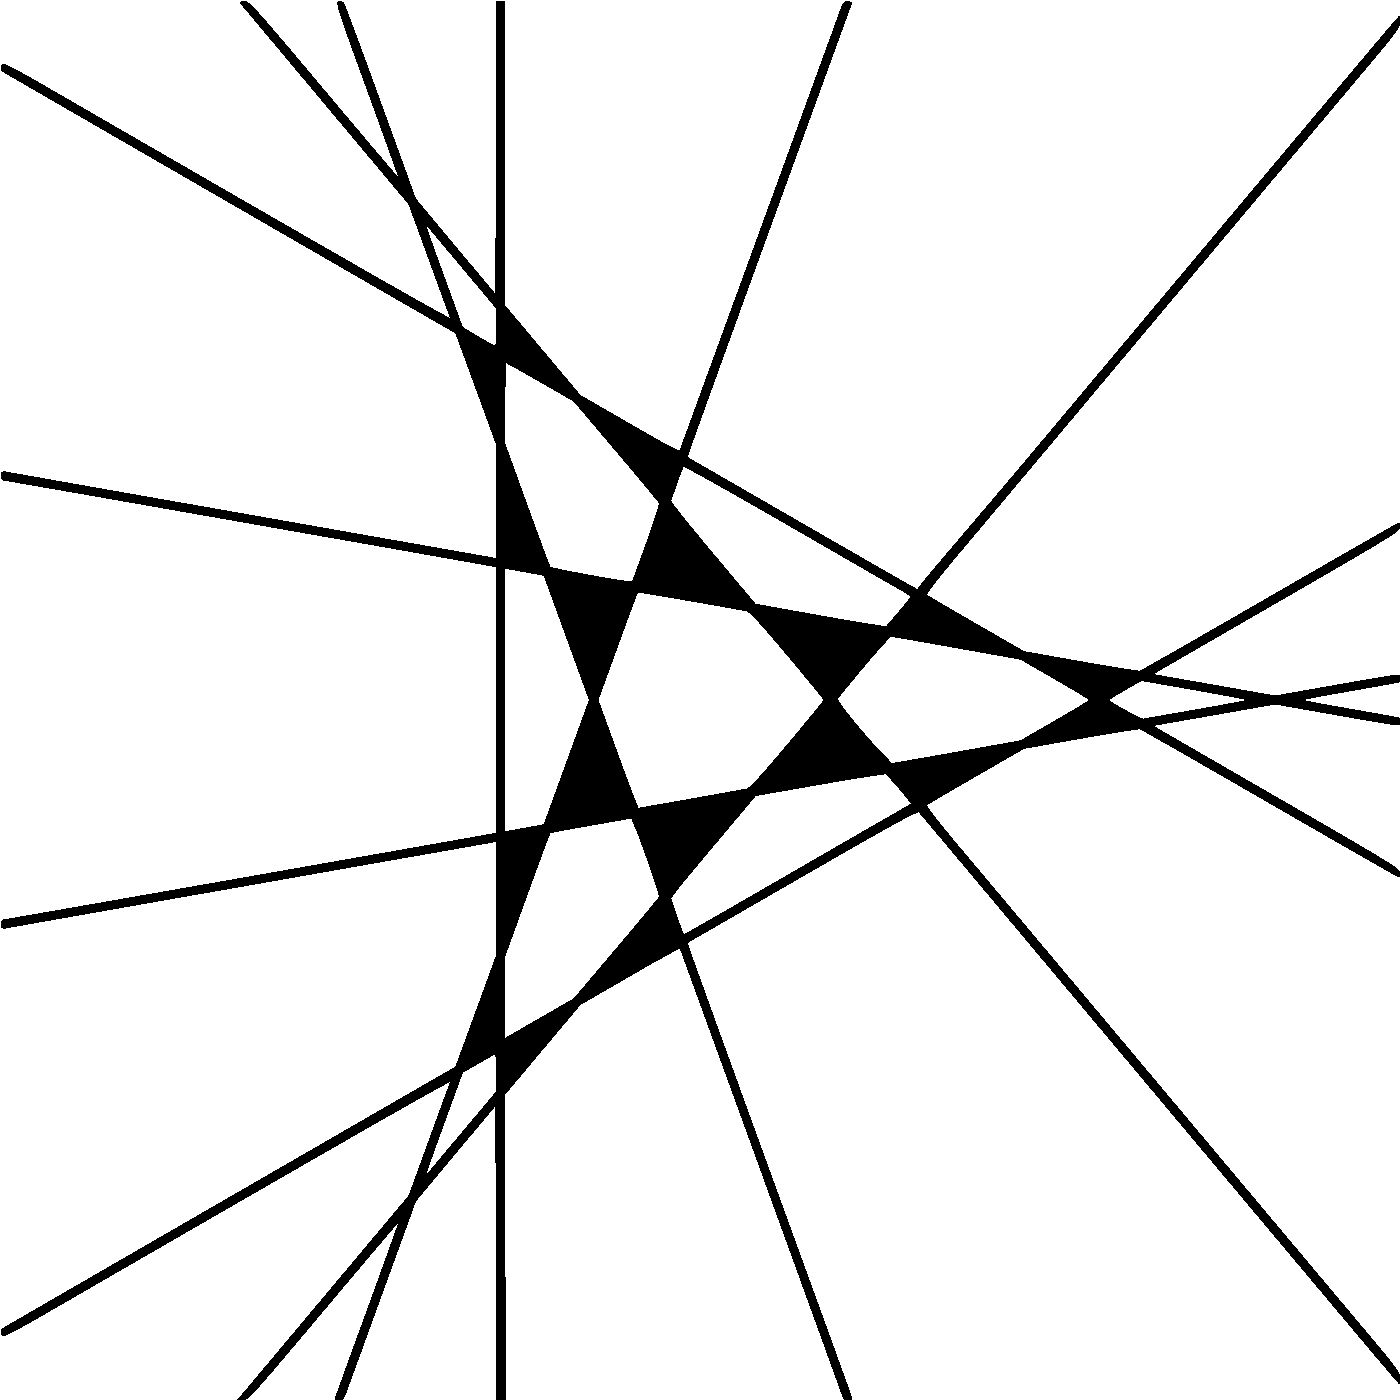
\includegraphics[height=1.5cm]{./../../common/images/vielesing.pdf}
        &
        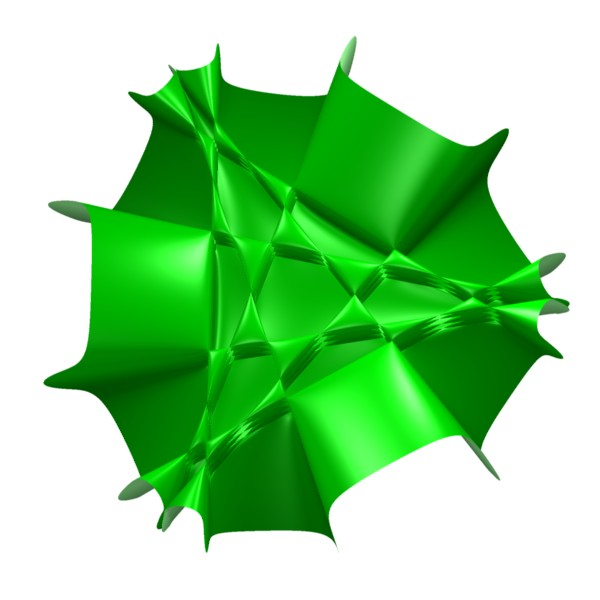
\includegraphics[height=1.5cm]{./../../common/images/p9surface_von_oben}
      \end{tabular}
    \end{center}
\end{surferPage}
